 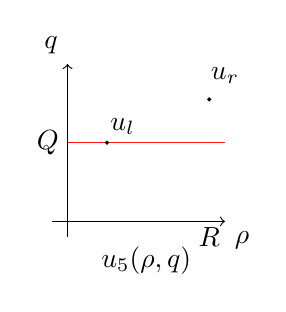
\begin{tikzpicture}
    % coordinates
    \draw[->] (0,-0.2) -- (0,2) node[anchor= south east] {$q$};
    \draw[->] (-0.2,0) -- (2,0) node[anchor= north west] {$\rho$};
    % disc
    \draw[red!90!white] (0,1) -- (2, 1);
    % contact disk
    %\draw[orange!50, domain=0:1.28]  plot[id=x] function{(x/1.16)*(2-1.16)/(2-x)*1.63};
    \draw[orange!50, domain=0:1.86]  plot[id=x] function{(x/1.38)*(2-1.38)/(2-x)*0.33};
    % initial conditions
    \node at (0.5+ 0.2, 1+0.2) {$u_l$};
    %\node at (1.06+0.2, 1.33+0.2) {$u_1$};
    %\node at (1.53+0.2, 0.48+0.2) {$u_{r_2}$};
    \node at (1.8+0.2, 1.55+0.3) {$u_{r}$};
    %\node at (0.77+0.2, 0.74+0.2) {$u_4$};
    \filldraw[black] (0.5, 1) circle (0.5pt);   % u_m
    %\filldraw[black] (0.77, 0.74) circle (0.5pt);   % u_m
    %\filldraw[black] (1.06, 1.33) circle (0.5pt);  % u_1
    %\filldraw[black] (1.53, 0.48) circle (0.5pt);   % u_2
    \filldraw[black] (1.8, 1.55) circle (0.5pt);   % u_m
    %labels
    \node at (1.8, -0.2) {$R$};
    \node at (-0.25, 1) {$Q$};
    \node at (1, -0.5) {$u_5(\rho,q)$};
    \end{tikzpicture}